\documentclass[12pt]{article}
\usepackage[T1]{fontenc}
\usepackage[utf8]{inputenc}
\usepackage[brazil]{babel}
\usepackage{graphicx}
\usepackage{hyperref}
\usepackage{fancyhdr}
\usepackage{background}
\usepackage[a4paper,top=3.5cm,left=3cm,right=3cm,bottom=2.5cm]{geometry}
\usepackage{lmodern}
\usepackage{tikz}
\usepackage[font={small,stretch=0.80,it}]{caption}
\usepackage{tcolorbox}

\newtcolorbox{caixa}{colback=red!5!white,colframe=red!75!black}

%Configurando o mapa mental
\usetikzlibrary{mindmap}

%Configurando a path das imagens
\graphicspath{{../../imagens/capitulo2/}}

%Configurando a imagem de background
\backgroundsetup{
scale=1,
angle=0,
opacity=0.4,
contents={%
  
\includegraphics[width=\paperwidth,height=\paperheight]{wallpaper.png}
  }%
}

%configurando os hyperlinks
\hypersetup{
    colorlinks=true,
    linkcolor=green,
    filecolor=magenta,      
    urlcolor=blue,
}

%configurando os headers
\pagestyle{fancy}
\fancyhf{}
\rhead{LDO}
\lhead{Capítulo 2}
\rfoot{Página \thepage}

%configurando identação e separação de parágrafos
\parindent 1.27cm
\parskip   6pt

%títulos,autor e data
\title{\textbf{Capítulo 2 \\ Novidades de Machine Learning na atualidade}}
\author{Gustavo Lopes Rodrigues}
\date{Novembro de 2020}

\begin{document}
    
    %Inserindo o título
    \maketitle

    \begin{center}
        \begin{tikzpicture}[mindmap, grow cyclic, every node/.style=concept, concept color=orange!40,
        level 1/.append style={level distance=5cm,sibling angle=90},
        level 2/.append style={level distance=3cm,sibling angle=45}]

        \node{Novidades em Machine Learning}
            child [concept color=blue!30] { node {GPT-3 \\ \ref{sec:gpt-3}}
                child { node {\href{https://www.sas.com/pt_br/insights/analytics/deep-learning.html}{Deep Learning}}}
                child { node {\href{https://openai.com/}{Open AI}}}
                child { node {\href{https://debuild.co/}{debuild.co}}}
            }
            child [concept color=yellow!30] { node {YouTube \\ \ref{sec:youtube}}
                child { node {\href{https://rockcontent.com/br/blog/algoritmo-do-youtube/}{Algoritmo de pesquisa}}}
                child { node {\href{https://youtu.be/oWcVTWLgACM}{Tags}}}
                child { node {\href{https://super.abril.com.br/tecnologia/como-funciona-a-recomendacao-de-videos-do-youtube/}{Recomen dação}}}
            }
            child [concept color=teal!40] { node {Amazon \\ \ref{sec:amazon}}
                child { node {\href{https://www.noticiastecnologia.com.br/amazon-ajusta-algoritmo-de-pesquisa-para-priorizar-os-proprios-produtos}{Relevância ou Lucro?}}}
                child { node {\href{https://www.visualcapitalist.com/amazon-worlds-most-valuable-retailer/}{Maior varejista dos EUA}}}
            }
            child [concept color=purple!50] { node {Deep Blue \\ \ref{sec:deep_blue}}
                child { node {\href{https://pt.wikipedia.org/wiki/Garry_Kasparov}{Garry Kasparov}}}
                child { node {\href{https://pt.wikipedia.org/wiki/IBM}{IBM}}}
                child { node {\href{https://canaltech.com.br/produtos/o-que-e-supercomputador/}{Super computador}}}
            };
        \end{tikzpicture}

    \end{center}

    %Configurando uma imagem
    \newpage    

    \begin{figure}[htp]

        \centering
        
\includegraphics[scale=0.3]{maxresdefault.jpg}
        \caption{\href{https://youtu.be/pbVwH8o837A}{Agora Aquela I.A. Foi Longe Demais (e vai mudar o jeito que você trabalha)}}

    \end{figure}
    
    \begin{caixa}

        \begin{center}

            \href{https://soundcloud.com/gustavo-rodrigues-468052117/ldo-machine-learning-capitulo02?in=gustavo-rodrigues-468052117/sets/ldo-machine-learning}{Ouça o Podcast desse PDF!}

        \end{center}

    \end{caixa}

    %Iniciando a seção 'Inicio'
    \section{Início} \label{sec:gpt-3}

    Eai? Você viu o vídeo acima do \href{https://br.linkedin.com/in/filipedeschamps}{Filipe Deschamps}? 
    Se não eu recomendo fortemente que assista, mas vamos comentar brevemente sobre o assunto 
    do mesmo: a GPT-3.

    Em Junho de 2020, a instituição de pesquisa em Inteligência Artificial,
    \href{https://openai.com/}{Open AI}, lançou as versões iniciais do Generative Pre-trained Transformer 3 também conhecido 
    pelo acrônimo GPT-3, que é um modelo de linguagem autoregressiva que usa 
    aprendizado profundo (\href{https://www.sas.com/pt_br/insights/analytics/deep-learning.html}
    {Deep Learning}) para produzir textos semelhantes aos humanos.

    Na primeira parte do vídeo, o primeiro exemplo dado foi do site \href{https://debuild.co/}{debuild.co} 
    que permite criar aplicativos web, rápidos apenas descrevendo as funcionalidades do programa. 
    Porém, como é demonstrado posteriormente pelo youTuber, a GPT-3 possui capacidades ainda mais 
    impressionantes, como: criar gráficos, criar planilhas ou até gerar textos de 
    figuras famosas, como \href{https://pt.wikipedia.org/wiki/Elon_Musk}{Elon Musk}.

    Isso é só um exemplo em como Machine Learning ainda é uma área que só tem 
    crescido desde o \href{../Capitulo_01/Capitulo01.pdf}{Game of Checkers}, mas não é 
    o único exemplo em como essa área da computação atua no nosso dia-a-dia.

    Um outro notável exemplo em como o Aprendizado de máquina tem evoluído é
    na área dos jogos.

    \newpage
    \section{Homem X Máquina} \label{sec:deep_blue}

    \begin{figure}[htp]
        \centering
        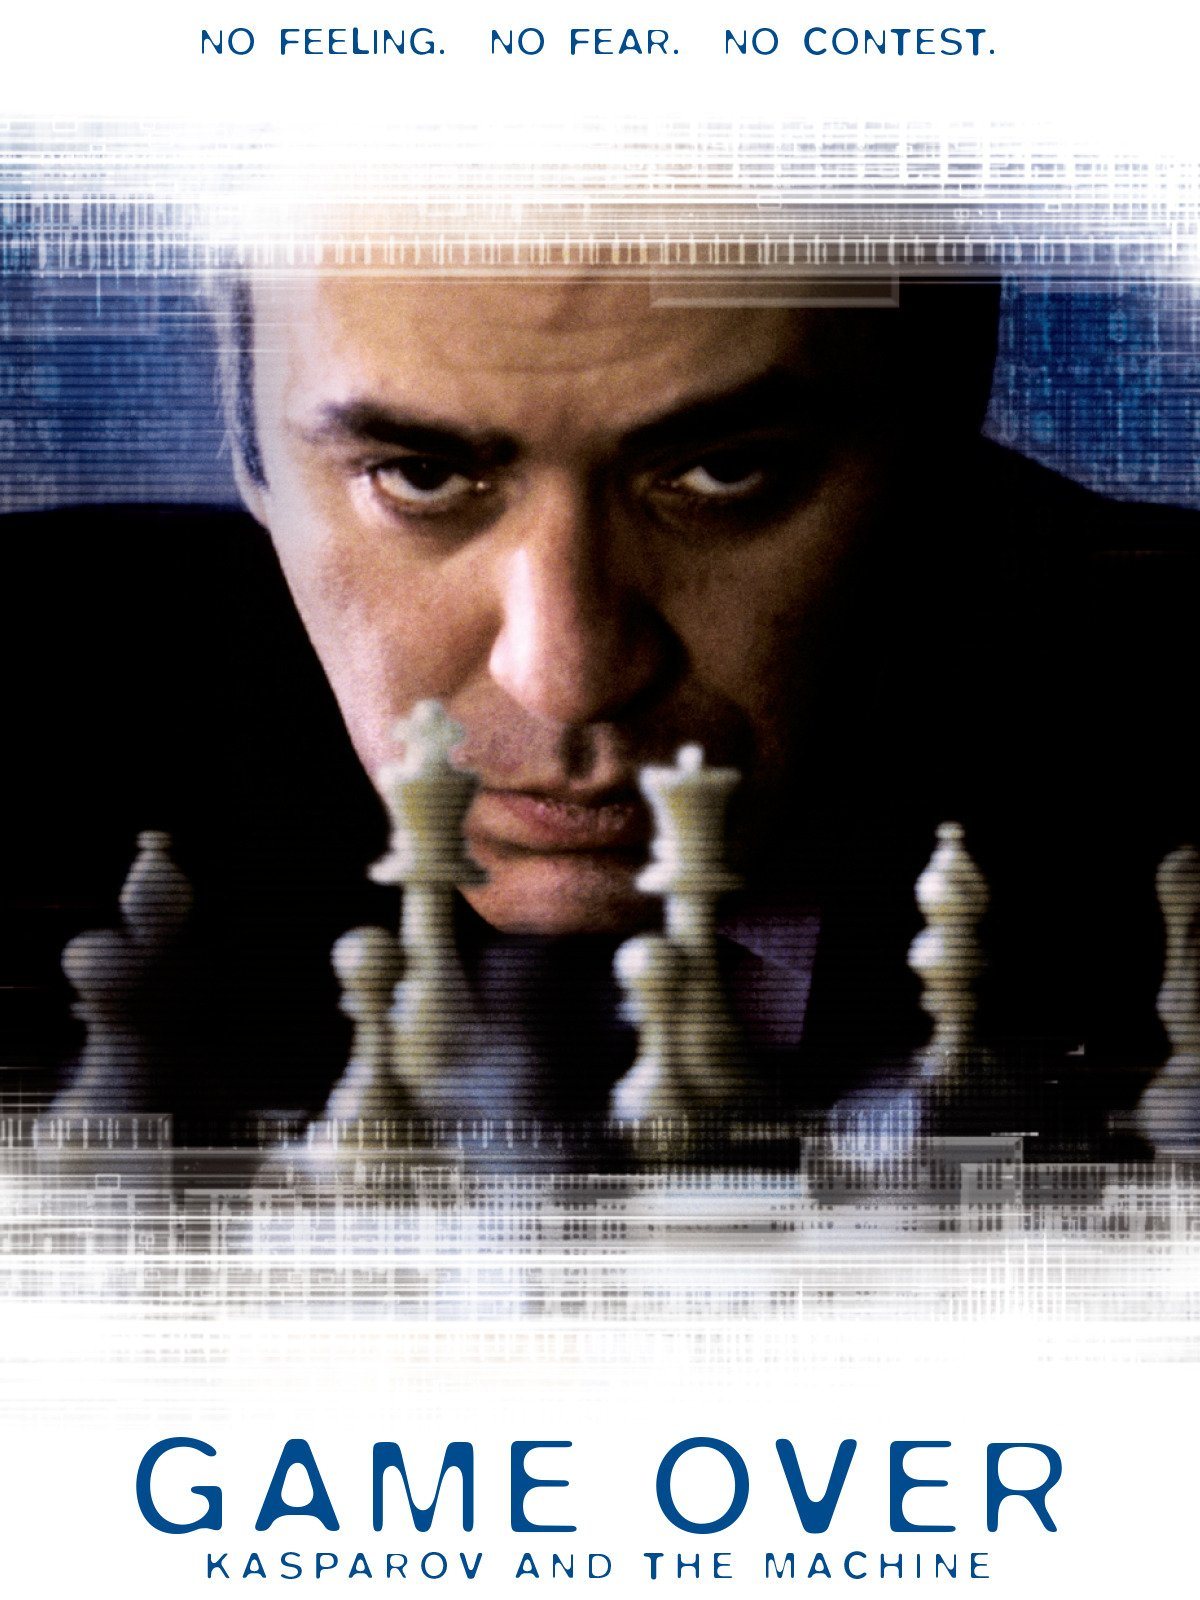
\includegraphics[scale=0.2]{GameOver.jpg}
        \caption{\centering Documentário sobre a partida entre Garry Kasparov e a Deep Blue}
    \end{figure}

    Em 1996 e 1997, \href{https://pt.wikipedia.org/wiki/Garry_Kasparov}{Garry Kasparov}, 
    na época o campeão mundial de xadrez foi desafiado
    a jogar contra a \href{https://pt.wikipedia.org/wiki/Deep_Blue}{Deep Blue}, um \href{https://canaltech.com.br/produtos/o-que-e-supercomputador/}{supercomputador} 
    criado pela \href{https://pt.wikipedia.org/wiki/IBM}{IBM} que foi designada especificamente para jogar xadrez. 

    Na primeira partida, o jogador da \href{https://pt.wikipedia.org/wiki/Uni%C3%A3o_Sovi%C3%A9tica}{União Soviética} 
    ganhou de 4 x 2, porém no ano seguinte, a IBM desafiou novamente Garry, agora com uma versão melhorada de sua tecnlogia. A 
    primeira versão era capaz de analisar 100 milhões de jogadas por segundo, o novo modelo era capaz
    de análisar até 250 milhões de jogadas!

    Dessa vez, a máquina ganhou de \(3\frac{1}{2}\) x \(2\frac{1}{2}\), marcando o momento histórico 
    onde pela primeira vez um jogador humano perdeu para uma máquina em um jogo.

    Vamos listar aqui dois exemplos,mas saiba que na seção \ref{sec:extra}, você encontrará mais links sobre o assunto “Machine Learning no cotidiano”, inclusive
    contendo mais exemplos sobre o aprendizado de máquinas em jogos, 

    %Forçar o programa ir para uma nova página
    \newpage
    \section{YouTube} \label{sec:youtube}

    \begin{figure}[htp]
        \centering
        
\includegraphics{youtube.png}
    \end{figure}

    Todos os vídeos na plataforma possuem uma característica muito importante
    que são: palavras-chave (também conhecida como ‘tags’). Quando você 
    assiste algum vídeo por um bom tempo, o algoritmo do YouTube irá induzir que 
    o usuário gosta do tipo de conteúdo que está no vídeo. Tendo isso em mente,
    ele irá pegar as palavras-chave do tal vídeo, e na próxima vez que o usuário 
    abrir a página de recomendação, os vídeos que estarão na lista serão 
    justamente aqueles que possuem as palavras-chave que o usuário demonstrou interesse.

    \newpage
    \section{Amazon} \label{sec:amazon}

    \begin{figure}[htp]
        \centering
        
\includegraphics[scale=0.3]{amazon.jpg}
    \end{figure}

    Assim como o YouTube, a Amazon também utiliza de um sistema de recomendações, 
    para direcionar produtos possivelmente relevantes a um cliente, mas além 
    disso, o sistema conta com um algoritmo que a partir de dados de pesquisas
    anteriores, o mesmo aprende o que é mais importante para os clientes na 
    hora de pesquisar determinado produto. Segundo estudos, quando tais 
    sistemas são colocados, \href{https://papers.ssrn.com/sol3/papers.cfm?abstract_id=2263983}
    {eles têm a capacidade de aumentar as compras em até 30\%}

    Em Setembro de 2019, a Amazon começou a ser suspeitada quanto ao seu algoritmo
    de busca, pois de acordo com \href{https://www.wsj.com/articles/amazon-changed-search-algorithm-in-ways-that-boost-its-own-products-11568645345}{matéria publicada no Wall Street Journal},
    o mesmo estava priorizando lucro em vez de relevância. De qualquer maneira, não é possível negar
    que a Amazon é umas das mais gigantes empresas da atualidade, sendo a maior
    varejista dos Estados Unidos, \href{https://www.visualcapitalist.com/amazon-worlds-most-valuable-retailer/}{de acordo com estudos}.


    \newpage
    \section{Conclusão}

    O restante dos exemplos, vamos deixar para a sua curiosidade. Mas acredito que 
    vocês tenham captado a ideia: Machine learning está em um contínuo uso dentro da 
    nossa sociedade e tem sido utilizado para melhorar a experiência dos usuários na internet, 
    direcionando a atenção dos usuários cibernéticos.

    Além disso, você também viu um pouco em como o Aprendizado de Máquina
    tem sido utilizado em jogos, provando que a máquina é capaz de até superar jogadores
    humanos! Se você se interessou pela leitura, recomendo fortemente que dê
    uma olhada no material extra que preparei, além de claro, continuar a sua leitura
    no \href{../Capitulo_03/Capitulo03.pdf}{\textbf{Capítulo 3}}.


    \newpage
    \section*{\centering Material extra}\label{sec:extra} %Criando uma tag para que possa ser referência em outras partes do programa

    %Iniciando listagem
    \begin{itemize}
        \item \href{http://datascienceacademy.com.br/blog/17-casos-de-uso-de-machine-learning/}{\textbf{Machine Learning no cotidiano}}
        \item \href{https://deepmind.com/research/case-studies/alphago-the-story-so-far}{\textbf{Alpha GO}} \\ Obs: \\ \href{https://youtu.be/WXuK6gekU1Y}{\textbf{Também de uma olhada no documentário sobre a Alpha GO}}
        \item \href{https://youtu.be/uGYJuOyIvzs}{\textbf{Aplicação de Machine Learning na saúde}}
        \item \href{https://youtu.be/AwmvwTopbas}{\textbf{Usando Machine Learning para fazer ampliação de vídeos}}
        \item \href{https://forbes.com.br/forbes-insider/2020/07/por-que-o-programa-de-inteligencia-artificial-gpt-3-e-incrivel-mas-superestimado/}{\textbf{Leia mais sobre a GPT-3!}}
    \end{itemize}

    \newpage

    %Iniciando referências
    \begin{thebibliography}{4}
        \bibitem{exemplos} 
        Equipe Interop \\
        \href{https://www.interop.com.br/blog/exemplos-de-machine-learning/}{\textbf{Exemplos de machine Learning}} 
        
        \bibitem{deschamps} 
        Filipe Deschamps \\
        \href{https://www.interop.com.br/blog/exemplos-de-machine-learning/}{\textbf{Agora Aquela I.A. Foi Longe Demais (e vai mudar o jeito que você trabalha)}}

        \bibitem{deepblue} 
        Deep Blue \\
        \href{https://pt.wikipedia.org/wiki/Deep_Blue}{\textbf{Artigo da Wikipedia sobre a Deep Blue}}
        
        \bibitem{deepblue} 
        Garry Kasparov X Deep Blue \\
        \href{https://pt.wikipedia.org/wiki/Deep_Blue}{\textbf{A história das partidas entre Garry Kasparov e Deep Blue}}
    \end{thebibliography}

    

\end{document}
